\chapter{实验背景及原理}
\label{cha:bg}
本章将在概论的基础上,基于实验目标,对实验原理进行简单阐述。

\section{实验目标}

\begin{itemize}
    \item 熟悉人脸检测及识别的基本原理和实现方法;
    \item 掌握基于 PCA 方法的人脸识别步骤 、 算法;
    \item 掌握主成分分析 、 特征值 、 特征脸的实现方法 获得对人脸识别的感性认识;
    \item 熟悉数字图像处理常用函数的使用方法及一般数字图像处理系统的设计方法;
    \item 学习 MATLB 软件实现 PCA 算法 进行人脸识别 加深其在其在数字图像处理中解决该类问题的应用流程
\end{itemize}

\section{实验原理概览}

完成本实验,需要了解图像数字化的基本知识。\textbf{从数学的角度出发},数字图片可以看作一个二元函数$f(x, y)$,其中$x, y$是图像的坐标,每组坐标代表着数字图片的一个“像素点”,而函数导出值$f$则是当前像素的强度数据(intensity value),通常来说是一个三元数据。因此,可以认为数字图片完成了二维平面向三维空间的投影。\cite{Tyagi_2018}\textbf{从信号的角度出发},可以将图像数字化看作是采样和量化两个空域处理的过程。采样是连续的二维模拟信号被离散为像素点的过程,量化则是连续的强度数据继续被离散为指定采样位(一般为8位)数据的过程。

本实验的灰度处理,正是对图片的颜色空间即强度数据进行研究。实验的滤波处理,则聚焦于噪声处理方向。实际上滤波还会被用于图像边缘特征、细节特征的增强,模糊处理、特征/频域水印等风格化处理。实验的主成分分析,则要运用到概率论和矩阵论的有关知识。

数字音频和数字图片在数学和信号角度上只有维数的区别,因此对他们的基础研究是相通的。数字处理除了在数学和信号处理中有重要意义外,还在信息提取、压缩、数据传输等各方面有着广泛的应用。

\section{子任务模块}

\subsection{图像的灰度处理}

花花世界无奇不有,但要将不同颜色通道的数据整合到一个通道,\inlinecite{Kanan_2012}指出也是具有挑战性的。下列给出实验中用到的三种由RGB通道取样到灰度通道的方式。(均不考虑伽马处理)

\begin{figure}[H]
    \centering
    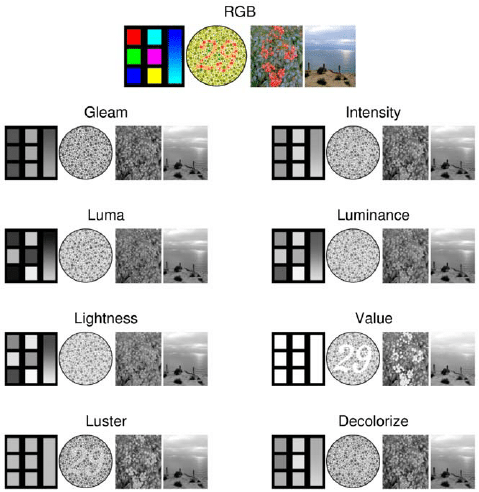
\includegraphics[width=.5\columnwidth]{the0.png}
    \caption{常见灰度处理方法及其应用结果\cite{Kanan_2012}}
    \label{fig:the0}
\end{figure}

\begin{itemize}
    \item 最大值取样(Value in HSV, Hue, Saturation, and Value)
    \begin{equation}
        G = \max \{R, G, B\}
    \end{equation}
    \item 平均值取样(Intensity)
    \begin{equation}
        G = \overline{ \{R, G, B\} }
    \end{equation}
    \item 加权平均值取样(Luminance, Follow CCIR 601)
    \begin{equation}
        G = 0.299 \cdot R + 0.587 \cdot G + 0.114 \cdot B
    \end{equation}\eqlist{Luma均值取样}[Luma均值取样]
\end{itemize}

\subsection{图像的滤波处理}

从频域上来看,滤波可分为低通和高通两种滤波类型。噪声可能是人为赋予,但更一般的情况下是感光元件和数据压缩处理时产生的,并一般在频域的高频段分布。故使用一些低通滤波可以减弱不同类型的噪声干扰。

\begin{figure}[H]
    \centering
    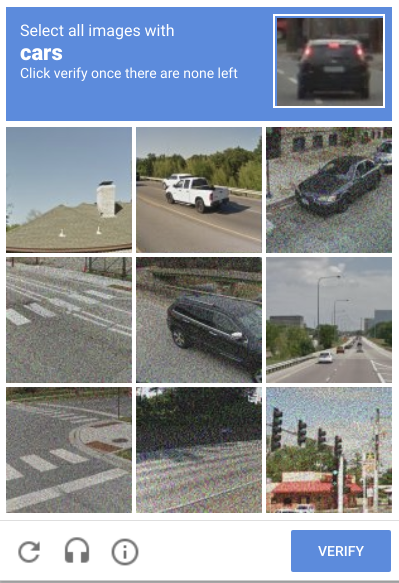
\includegraphics[width=.5\columnwidth]{the1.png}
    \caption{在验证码的识别图像中出现的对抗噪声(Adversarial Noise)\cite{Lambda_2018}}
    \label{fig:the1}
\end{figure}

本实验中用到了三种滤波方法:设$f(i, j)$表示$(i, j)$所代表的像素点的强度数据,$k$表示滤波在二维空域上的应用范围。实验时均使用的是小滤波子(即$k=1$)。

\subsubsection{均值滤波}
\label{sec:mean-filter0}

当$k=1$时,均值滤波可表示为:

\begin{alignat}{3}
    f(i, j) =& \rm{mean} \{& \forall{i_0, j_0} \in \{ x \in {Z} | &  -k \leq x \leq k\}~&~f(i + i_0, j + j_0)\}\\
    =&\rm{mean} \{& f(i - 1, j - 1),& f(i - 1, j),& f(i - 1, j + 1)\notag\\
    && f(i, j - 1),& f(i, j),& f(i, j + 1)\notag\\
    && f(i + 1, j - 1),& f(i + 1, j),& f(i + 1, j + 1)\}\notag
\end{alignat}

均值滤波(mean filter)常用于图像平滑和模糊,对随机噪声的去除性好。

\subsubsection{中值滤波}
\label{sec:median-filter0}

当$k=1$时,中值滤波可表示为:
\begin{alignat}{3}
    f(i, j) =& \rm{med} \{& \forall{i_0, j_0} \in \{ x \in {Z} | &  -k \leq x \leq k\}~&~f(i + i_0, j + j_0)\}\\
    =&\rm{med} \{& f(i - 1, j - 1),& f(i - 1, j),& f(i - 1, j + 1)\notag\\
    && f(i, j - 1),& f(i, j),& f(i, j + 1)\notag\\
    && f(i + 1, j - 1),& f(i + 1, j),& f(i + 1, j + 1)\}\notag
\end{alignat}\eqlist{中值滤波}[中值滤波]

中值滤波(median filter)可有效除去脉冲噪声,如\autoref{sec:dataset}中描述的数据集。\cite{Arakawa_1996}

\subsubsection{高斯滤波}
\label{sec:gaussian-filter0}

高斯滤波核可由下式计算:

\begin{equation}
    f(i,j) =\frac{1}{2\pi\sigma^2}e^{-\frac{i^2+j^2}{2\sigma^2}}
\end{equation}

高斯滤波(mean filter)也常用于图像平滑和模糊,对频域高斯噪声的去除性好。此处的高斯滤波为低通高斯滤波。

\subsection{图像的主成分分析}

\subsubsection{协方差矩阵}

协方差各项为$Cov(\vec x, \vec y)$。此处不考虑协方差矩阵的系数。

可证得协方差矩阵的特征向量按特征值从大到小排序后,各向量归一化(normalization, 2-范数为零)后得到的矩阵即为到主成分空间的变换矩阵。

\subsubsection{变换矩阵的计算}

鉴于数据规模大,我们需要使用矩阵SVD分解的知识来快速、省空间地得到主成分空间的变换矩阵,即原矩阵的协方差矩阵的特征向量矩阵(经排序和归一化处理)。

首先对矩阵中心化(centralization)处理,这使得\autoref{align:import}结果是方差相乘,满足协方差矩阵的定义。(此处数据都是行向量)

\begin{align}
    X_{c(m\times n)} &= X_{m\times n} - \overline{X_{m\times 1}} \cdot [1]_{1\times n} \\
    Cov_{n \times n} &= X^T_c \cdot X_c \label{align:import}
\end{align}

若真要这么计算,n所代表的高维数将让计算机难以下手。但由SVD分解知识可得(此处省略系数):

\begin{align}
\begin{split}
    \rm{eig}(Cov_{n \times n}) &= \\
    \rm{eig}(X^T_c \cdot X_c) &= X_C \cdot \rm{eig}(X_c \cdot X^T_c)
\end{split}
\end{align}\eqlist{SVD导出}[SVD导出]

至此,求出$ T_{m \times m} = X_c \cdot X^T_c $,再进行特征值求解(Listing \ref{listing:dev}),便可以将高维图片向量组乘以变换矩阵,得到各向量降维后的各主成分了。\cite{Abdi_2010, orfanidis_2007, Wold_1987, Pearson_1901}

另外,由于要用到的主成分空间维数不高,还有人提出贪心的算法优化计算。\cite{王晓伟_2013}

\subsubsection{样本分类方法}

k近邻算法(kNN, k Nearest Neighbor)在非监督学习(聚类)中称为k平均算法,其计算样本到各数据点的欧式距离,并选择距离最近的k个数据点,将出现最多的类别作为样本所属分类。该分类算法效果依赖于选择的k值,且因其懒惰学习的特性,导致分类效率低。\textbf{本实验没有采用kNN的任何优化变种,同时出现多个最大值时对k进行缩小迭代},其中欧氏距离:\cite{Guo_2003}

\begin{equation}
    d = \Vert\vec x - \vec y\Vert = \sqrt{\sum^{n}_{i=1} {(x_i - y_i)}^2}
\end{equation}


注意到该方案和近邻成分分析(NCA, Neighbourhood components analysis)原理虽然相似,但缺少状态估计环节和梯度分析。

该方案用于给定数据及标签,对样本进行分类的任务,故此时的kNN分类算法充当着有监督学习的工具。

除了使用kNN分类算法,支持向量机(SVM)也经常用于对数据更主动的分类,且预期效果比人工对$k$调参要好得多。\cite{Cortes_1995, techping_2018, Hu_2019}